\def\i{\item}
\graphicspath{{../pictures/c5/}}
%\chapter{MỘT SỐ YẾU TỐ THỐNG KÊ VÀ XÁC SUẤT}
\newpage
\section{ỨNG DỤNG XÁC SUẤT TRONG THỰC TIỄN CÁC KIẾN THỨC CẦN NHỚ}
\subsubsection{Kết quả có thể và sự kiện trong trò chơi, thí nghiệm}
\begin{enumerate}[--,leftmargin=*]
	\i Kết quả có thể: các kết quả của trò chơi, thí nghiệm có thể xảy ra gọi là kết quả có thể.
	\i Sự kiện: Khi thực hiện trò chơi hoặc thí nghiệm, một sự kiện có thể xảy ra hoặc không xảy ra tùy thuộc vào kết quả của trò chơi, thí nghiệm đó.
\end{enumerate}
\subsubsection{Xác suất thực nghiệm} 
Thực hiện lặp đi lặp lại một hoạt động nào đó $n$ lần. Gọi $n(A)$ là số lần sự kiện $A$ xảy ra trong $n$ lần đó. Tỉ số
\[\dfrac{n(A)}{n} = \dfrac{\text{Số lần sự kiện $A$ xảy ra}}{\text{Tổng số lần thực hiện hoạt động}}\] 
được gọi là \textit{xác suất thực nghiệm} của sự kiện $A$ sau $n$ hoạt động vừa thực hiện.

\textbf{Nhận xét:} Xác suất thực nghiệm phụ thuộc vào người thực hiện thí nghiệm, trò chơi và số lần người đó thực hiện thí nghiệm, trò chơi.
\subsection{THỰC HÀNH GIẢI TOÁN}
\begin{vd}
	Trong một hộp có 1 bút đen, 1 bút xanh, 1 bút đỏ. Hãy liệt kê và viết tập hợp các kết quả có thể của mỗi hoạt động sau: 
	\begin{enumerate}[a),leftmargin=*]
		\i Lấy ra một bút từ hộp.
		\i Lấy ra cùng lúc 2 bút từ hộp.
	\end{enumerate}
	\loigiai{
		\begin{enumerate}[a),leftmargin=*]
			\i Lấy ra một bút từ hộp có 1 bút đen, 1 bút xanh, 1 bút đỏ. \\
			Các khả năng có thể xảy ra như sau: khả năng lấy ra 1 bút  đen, khả năng lấy ra 1 bút xanh, khả năng lấy ra 1 bút đỏ. \\
			Tập hợp tất cả các kết quả có thể xảy ra của hoạt động 1 là:  
			\[A = \{1 bút đen, 1 bút xanh, 1 bút đỏ\}\]
			số phần tử là 3.
			\i Lấy ra cùng lúc 2 bút từ hộp có 1 bút đen, 1 bút xanh, 1 bút đỏ. Các khả năng có thể xảy ra như sau:   
			\begin{enumerate}[+,leftmargin=*]
				\i khả năng lấy ra 1 bút đen và 1 bút xanh (ĐX)
				\i khả năng lấy ra 1 bút đen và 1 bút đỏ (ĐĐo)
				\i khả năng lấy ra 1 bút xanh và  1 bút đỏ (XĐo) 
			\end{enumerate}
			Tập hợp tất cả các kết quả có thể xảy ra $B = \{\text{ĐX, Đđo, XĐo}\}$, số phần  tử là 3.
		\end{enumerate}
	}
\end{vd}
\begin{vd}
	Gieo một con xúc xắc sáu mặt và quan sát mặt xuất hiện của nó.
	\begin{enumerate}[a),leftmargin=*]
		\i Sự kiện nào sau đây có thể xảy ra:
		\begin{enumerate}[(1),leftmargin=*]
			\i Số chấm xuất hiện trên con xúc xắc là số lẻ.
			\i Số chấm xuất hiện trên con xúc xắc lớn hơn 7.
			\i Số chấm xuất hiện trên con xúc xắc lớn hơn 4.
			\i Số chấm xuất hiện trên con xúc xắc chia hết cho 3.
			\i Số chấm xuất hiện trên con xúc xắc là số nguyên tố.
		\end{enumerate}
		\i Hãy viết tập hợp các kết quả có thể xảy ra với mỗi sự kiện (nếu có) ở trên.
	\end{enumerate}
	\loigiai{
		\textbf{Tìm cách giải:}
		\begin{enumerate}[a),leftmargin=*]
			\i Khi liệt kê tất cả các kết quả có thể xảy ra khi gieo con xúc xắc ta có: 1, 2, 3, 4, 5, 6.\\
			Từ đó thấy rằng sự kiện (2) không thể xảy ra. Các sự kiện (1), (3), (4), (5) có thể xảy ra.
			\i Dễ dàng liệt kê được từ tập hợp  $\{1.2.3.4.5.6\}$
			\begin{enumerate}[--,leftmargin=*]
				\i Các số lẻ là:  1, 3 ,5.
				\i Các số lớn hơn 4 là:  5; 6.
				\i Các số chia hết cho 3 là: 3; 6. 
				\i Các số nguyên tố là: 2;3;5.
			\end{enumerate}
		\end{enumerate} 
		\textbf{Trình bày lời giải:}
		\begin{enumerate}[a),leftmargin=*]
			\i Các sự kiện (1), (3), (4), (5) có thể xảy ra.
			\i \begin{enumerate}[--,leftmargin=*]
				\i Với sự kiện (1), tập hợp các kết quả có thể xảy ra là: $X_1 = \{1;3;5\}$.
				\i Với sự kiện (3), tập hợp các kết quả có thể xảy ra là:  $X_3 = \{5; 6\}$.
				\i Với sự kiện (4), tập hợp các kết quả có thể xảy ra là:  $X_4 = \{3;6\}$.
				\i Với sự kiện (5), tập hợp các kết quả có thể xảy ra là:  $X_5 = \{2;3;5\}$.
			\end{enumerate}
		\end{enumerate}
	}
\end{vd}
\begin{vd}
	Hãy liệt kê các kết quả có thể xảy ra của hoạt động tung đồng thời hai đồng xu.
	\loigiai{
		\textbf{Tìm cách giải:}
		\begin{enumerate}[--,leftmargin=*]
			\i Nêu các kết quả có thể xảy ra khi tung một đồng xu?
			\i Khi tung đồng thời hai đồng xu thì các kết quả có thể xảy ra là gì?
		\end{enumerate}
		\textbf{Trình bày lời giải:}
		\begin{enumerate}[--,leftmargin=*]
			\i Khi tung đồng thời hai đồng xu thì các kết quả có thể xảy ra là: SS, NN, SN, NS (S: Sấp, N: Ngửa)
		\end{enumerate}
		\textbf{\textit{$^*$Sai lầm thường gặp:}} Nhiều người chỉ liệt kê 3 kết quả có thể là: 2 sấp, 2 ngửa, 1 sấp 1 ngửa. Thực chất "1 sấp 1 ngửa" là một sự kiện mà không phải là một kết quả có thể. Sự kiện này gồm 2 kết quả có thể là SN, NS (N: Ngửa, S: Sấp).
		
		\textbf{\textit{$^*$Nhận xét:}} Bài toán về kết quả có thể và sự kiện trong các trò chơi, thí nghiệm sử dụng đếm và liệt kê các phần tử của một tập hợp.
	}
\end{vd}
\begin{vd}
	Minh tung cùng một lúc hai đồng xu 20 lần và ghi lại kết quả như sau: 
	\begin{center}
		\begin{tabular}{|c|c|c|c|}
			\hline
			Sự kiện&	Hai đồng sấp&	Một đồng sấp, một đồng ngửa&	Hai đồng ngửa\\
			\hline
			Số lần&	6&	12&	4\\
			\hline
		\end{tabular}
	\end{center}
	Tính xác suất thực nghiệm của sự kiện Một đồng sấp, một đồng ngửa.
	\loigiai{
		\textbf{Tìm lời giải:}
		\begin{enumerate}[--,leftmargin=*]
			\i Xác định số lần thực hiện hoạt động.
			\i Xác định số lần sự kiện "Một đồng sấp, một đồng ngửa" xảy ra.
			\i Áp dụng công thức tính xác suất thực nghiệm.
		\end{enumerate}
		\textbf{Trình bày lời giải:}
		Số lần Minh tung cùng một lúc hai đồng xu là: $n = 20.$
		
		Số lần xuất hiện một đồng sấp, một đồng ngửa là: $n(SN) = 12$
		 
		Xác suất thực nghiệm của sự kiện \textit{Một đồng sấp, một đồng ngửa} là:
		\[\dfrac{{n(SN)}}{n} = \dfrac{{12}}{{20}} = 60\%\] 
	}
\end{vd}
\begin{vd}
	Minh gieo một con xúc xắc 100 lần và ghi lại số chấm xuất hiện ở mỗi lần gieo được kết quả như sau:
	\begin{center}
		\begin{tabular}{|l|c|c|c|c|c|c|}
			\hline
			Số chấm xuất hiện&	1&	2&	3&	4&	5&	6\\
			\hline
			Số lần&	15&	20&	18&	22&	10&	15\\
			\hline
		\end{tabular}
	\end{center}
	Tính xác suất thực nghiệm của các sự kiện sau:
	\begin{enumerate}[a),leftmargin=*]
		\i Số chấm xuất hiện là số nguyên tố.
		\i Số chấm xuất hiện là hợp số.
	\end{enumerate}
	\loigiai{
		\textbf{Tìm lời giải:}
		\begin{enumerate}[--,leftmargin=*]
			\i Xác định số lần thực hiện hoạt động.
			\begin{enumerate}[a),leftmargin=*]
				\i Trong các số chấm xuất hiện, số nào là số nguyên tố?
				\begin{enumerate}[+,leftmargin=*]
					\i Số lần xuất hiện mặt 2 chấm; 3 chấm; 5 chấm chính là số lần số chấm xuất hiện là số nguyên tố.
				\end{enumerate}
				\i Trong các số chấm xuất hiện, số nào là hợp số?
				\begin{enumerate}[+,leftmargin=*]
					\i Số lần xuất hiện mặt 4 chấm; 6 chấm chính là số lần số chấm xuất hiện là hợp số.
					\i Áp dụng công thức tính xác suất thực nghiệm.
				\end{enumerate}
			\end{enumerate}
		\end{enumerate}
		\textbf{Trình bày lời giải:}
		Số lần Minh thực hiện gieo xúc xắc là:  $n = 100$.
		\begin{enumerate}[a),leftmargin=*]
			\i Số lần số chấm xuất hiện là số nguyên tố là:  $n(NT) = 20 + 18 + 10 = 48$.\\
			Xác suất thực nghiệm của sự kiện \textit{Số chấm xuất hiện là số nguyên tố} là: 
				\[\dfrac{{n(NT)}}{n} = \dfrac{{48}}{{100}} = 48\%\]
			\i Số lần số chấm xuất hiện là hợp số là:  $n(H{\rm{S}}) = 22 + 15 = 37$\\
			Xác suất thực nghiệm của sự kiện \textit{Số chấm xuất hiện là hợp số} là: 
			\[\dfrac{{n(H{\rm{S}})}}{n} = \dfrac{{37}}{{100}} = 37\%\]
		\end{enumerate}
		\textbf{\textit{$^*$Sai lầm thường gặp:}} Học sinh nhầm mặt 1 chấm là hợp số, nên yêu cầu học sinh nhắc lại định nghĩa số nguyên tố, hợp số (đều là số tự nhiên lớn hơn 1) trước khi làm bài.
		
		\textbf{\textit{$^*$Nhận xét:}} Để tính xác suất thực nghiệm áp dụng công thức:
		\[\dfrac{n(A)}{n} = \dfrac{\text{Số lần sự kiện $A$ xảy ra}}{\text{Tổng số lần thực hiện hoạt động}}\]
	}
\end{vd}
\subsection{MỞ RỘNG KIẾN THỨC}
\subsubsection*{Thú vị cách nhà toán học Anh dùng xác suất giải bài toán tình báo của quân Đức trong thế chiến II}
Bắt đầu từ tháng 6 năm 1944, Miền nam nước Anh là mục tiêu tấn công liên tiếp của quân Đức bằng “Bom Bay – V1” – Tiền thân của các tên lửa hành trình. Các cuộc tấn công diễn ra trong suốt mùa hè với mục đích làm tiêu hao sinh lực của quân Đồng Minh. Hitler sở hữu những căn cứ ở Pháp và Hà Lan, có thể dễ dàng biến London thành bia ngắm với những trái bom này. Theo thống kê, chỉ trong 4 tháng, quân Đức đã phóng hơn 9500 quả V-1, và 25\% số bom đó được “ưu ái” dành tặng cho London.

Vấn đề lớn đối với ban chỉ huy quân Đồng Minh ngay lúc này là xác định xem kẻ thù có sở hữu một loại vũ khí hay tin tình báo quan trọng nào không. Bởi vì các địa điểm bị oanh tạc nhạy cảm có số lượng bom tập trung rất đáng ngờ. Và rắc rối lớn nhất là nếu Quân đôi Đức biết chính xác vị trí cần ném bom thì nguy cơ có lỗ hổng tình báo trong hệ thống là rất cao.

Vậy làm sao để biết được quân Đức đang ném bom có chủ đích hay chỉ đơn thuần là rải bom một cách ngẫu nhiên? Đáp án lại đến từ các nhà toán học. Tình báo Anh rất thận trọng trong việc theo dõi thời gian và vị trí bị V-1 oanh tạc. Và sau đó một nhà toán học được yêu cầu bí mật phân tích một mẩu giấy ghi chi chít những điểm đen trên toàn London.

Hai năm sau tháng 6 định mệnh đó, nhà toán học  R. D. Clarke đã lần đầu tiết lộ công chúng những khảo sát ông từng làm để giúp đỡ quân Đồng Minh. Sau khi được yêu cầu nghiên cứu quy luật ném bom, Clarke chia một khu vực rộng 12 x 12km  thành 576 ô vuông bằng nhau. Nơi đây có 537 quả bom được thả. Ông tính toán xem từng ô vuông có bao nhiêu quả bom rơi trúng, sau đó đánh giá mật độ và vẽ lên một biểu đồ phân bố bom rơi

Trong biểu đồ chúng ta có thể thấy những vùng trung tâm bị rơi nhiều bom nhất – 5 quả trên mỗi đơn vị diện tích, càng ở biên thì mức độ tàn phá cũng giảm dần. Nếu là một người ngoài nghề dùng cái nhìn cảm tính thì có thể đoán rằng, quân Đức đang tấn công có mục đích vào các vị trí trọng điểm. Nhưng thực ra không phải vậy. Trên thực tế khi phân tích số liệu, Clarke phát hiện ra rằng số lượng bom được phân phối trong biểu đồ tương tự như phân phối Poisson.
\begin{figure}[H]
	\centering
	\vspace*{-5pt}
	\captionsetup{labelformat= empty, justification=centering}
	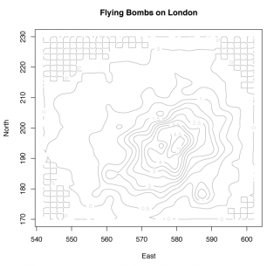
\includegraphics[width=0.5\linewidth]{15}
	\vspace*{-10pt}
\end{figure}
Điều này có nghĩa là, bom rơi tự nhiên, người Đức chỉ đơn giản là thả bom vu vơ mà chẳng có chút thông tin tình báo gì. Quân đồng minh có thể thở phào nhẹ nhõm!
\subsection{BÀI TẬP TỰ LUYỆN}
\Opensolutionfile{loigiaichung}[loigiaichuong41]
\subsubsection*{Mức độ cơ bản}
\begin{bt}
	Trong một hộp có 1 bút đen, 1 bút xanh, 1 bút đỏ. Hãy viết tập hợp các kết quả có thể của mỗi hoạt động sau: 
	\begin{enumerate}[a),leftmargin=*]
		\i Lấy ra từ hộp lần lượt (không thả lại) 2 chiếc bút.
		\i Lấy ra từ hộp lần lượt (không thả lại) 3 chiếc bút.
	\end{enumerate}
	\begin{loigiaichuong41}
		\begin{enumerate}[a),leftmargin=*]
			\i $X_1 = \{\text{ĐX; ĐĐo; XĐ; XĐo; ĐoĐ; ĐoX}\}$
			\i $X_2 = \{\text{ĐXĐo; ĐĐoX; XĐĐo; XĐoĐ; ĐoĐX; ĐoXĐ}\}$
		\end{enumerate}
	\end{loigiaichuong41}
\end{bt}
\begin{bt}
	Viết tập hợp sự kiện có thể xảy ra trong hoạt động tung đồng thời hai đồng xu.	
	\begin{loigiaichuong41}
	$\{$2 sấp; 2 ngửa; 1 sấp 1 ngửa$\}$
	\end{loigiaichuong41}
\end{bt}
\begin{bt}
	Lớp $6A$ tổ chức trò chơi "Vòng tròn lí thú", trong đó vòng quay hình tròn được chia thành tám phần bằng nhau và được đánh số điểm lần lượt từ 10 đến 80 như hình bên.
	\begin{figure}[H]
		\centering
		\vspace*{-5pt}
		\captionsetup{labelformat= empty, justification=centering}
		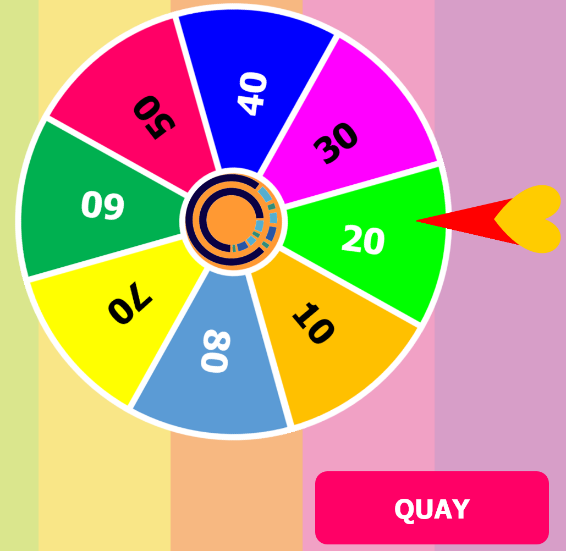
\includegraphics[width=0.35\linewidth]{16}
		\vspace*{-10pt}
	\end{figure}
	Quay vòng tròn 1 lần.
	\begin{enumerate}[a),leftmargin=*]
		\i Liệt kê các kết quả có thể xảy ra đối với số ở vòng tròn mà chiếc kim chỉ vào khi vòng tròn dừng lại.
		\i Liệt kê các kết quả có thể để sự kiện \textit{Mũi tên không chỉ vào ô 80 điểm} xảy ra;
		\i Nếu mũi tên chỉ vào ô 20 điểm như hình vẽ thì sự kiện \textit{Mũi tên chỉ vào ô 20 hoặc 50} có xảy ra không?
	\end{enumerate}
	\begin{loigiaichuong41}
		\begin{enumerate}[a),leftmargin=*]
			\i Có 8 kết quả có thể: 10; 20; 30; 40; 50; 60; 70; 80.
			\i 10; 20; 30; 40; 50; 60; 70.
			\i Sự kiện xảy ra.
		\end{enumerate}
	\end{loigiaichuong41}
\end{bt}
\begin{bt}
	Nhi lấy ra một quả bóng từ trong hộp có chứa 4 quả bóng xanh, 3 quả bóng đỏ, 3 quả bóng vàng.
	\begin{enumerate}[a),leftmargin=*]
		\i Liệt kê tất cả các sự kiện có thể xảy ra.
		\i Sự kiện “Nhi lấy được quả bóng màu xanh” có luôn xảy ra không?
		\i Tính xác suất lấy được quả bóng màu xanh.
	\end{enumerate}
	\begin{loigiaichuong41}
		\begin{enumerate}[a),leftmargin=*]
			\i Các sự kiện có thể xảy ra là: Nhi lấy ra được quả bóng màu xanh, Nhi lấy ra được quả bóng màu đỏ hoặc Nhi lấy ra được quả bóng màu vàng.
			\i Sự kiện “Nhi lấy được quả bóng màu xanh” không luôn xảy ra vì có thể quả bóng Nhi lấy ra có màu đỏ hoặc màu vàng.
			\i Xác suất lấy được quả bóng màu xanh là: $\dfrac{4}{{4 + 3 + 3}} = \dfrac{2}{5}$
		\end{enumerate}
	\end{loigiaichuong41}
\end{bt}
\begin{bt}
	Khi gieo đồng thời hai con xúc xắc sáu mặt cân đối và đồng chất. Quan sát số chấm xuất hiện trên mỗi con xúc xắc. Hãy đánh giá xem mỗi sự kiện sau là chắc chắn xảy ra, không thể xảy ra, hay có thể xảy ra.
	\begin{enumerate}[a),leftmargin=*]
		\i Tổng số chấm xuất hiện trên hai con xúc xắc bằng 1.
		\i Tích số chấm xuất hiện trên hai con xúc xắc bằng 1.
		\i Tổng số chấm xuất hiện trên hai con xúc xắc lớn hơn 1.
		\i Hai mặt xuất hiện cùng số chấm.
	\end{enumerate}
	\begin{loigiaichuong41}
		\begin{enumerate}[a),leftmargin=*]
			\i Sự kiện không thể xảy ra.
			\i Sự kiện không thể xảy ra..
			\i Sự kiện chắc chắn xảy ra.
			\i Sự kiện có thể xảy ra.
		\end{enumerate}
	\end{loigiaichuong41}
\end{bt}
\begin{bt}
	Trong đại hội chi đội lớp 6A, danh sách bầu ban cán sự lớp cho vị trí lớp trưởng gồm 4 bạn: Thanh, Ly, Chính, Linh.
	Trong đó chỉ có Chính là nam.
	\begin{enumerate}[a),leftmargin=*]
		\i Em có chắc chắn bạn nào sẽ là lớp trưởng không?
		\i Một bạn trong lớp nói rằng “ Lớp trưởng lớp mình chắc chắn là một bạn nữ”.\\
		Em có nghĩ là bạn đó nói đúng không?
		\i Hãy liệt kê các kết quả có thể để sự kiện “Lớp trưởng không phải là Chính” xảy ra.
	\end{enumerate}
	\begin{loigiaichuong41}
		\begin{enumerate}[a),leftmargin=*]
			\i Không chắc chắn được bạn nào sẽ là lớp trưởng.
			\i Bạn đó nói chưa chắc đúng vì lớp trưởng có thể là Chính (bạn nam).
			\i Kết quả có thể để sự kiện "Lớp trưởng không phải là Chính" xảy ra là: Thanh, Ly, Linh.
		\end{enumerate}
	\end{loigiaichuong41}
\end{bt}
\begin{bt}
	Trong hộp có 20 viên bi gồm 10 viên bi xanh, 6 viên bi đỏ và 4 viên bi vàng. Lấy ngẫu nhiên 1 viên bi. Tính xác xuất thực nghiệm lấy được viên bi:
	\begin{center}
		a) Màu xanh         \quad\quad\quad    b) Màu đỏ       \quad\quad\quad                   c) Màu vàng
	\end{center}
	\begin{loigiaichuong41}
			a) $\dfrac{n(X)}{n} = \dfrac{10}{20} = 50\%$\quad\quad
			b) $\dfrac{n(Đ)}{n} = \dfrac{6}{20} = 30\%$\quad\quad
			c) $\dfrac{n(V)}{n} = \dfrac{4}{20} = 20\%$
	\end{loigiaichuong41}
\end{bt}
\begin{bt}
	Khi gieo một đồng xu 15  lần. Nam thấy có  9 lần xuất hiện mặt ngửa (N). Hãy tính xác suất thực nghiệm của sự kiện mặt sấp (S) xuất hiện.
	\begin{loigiaichuong41}
		$\dfrac{{n(S)}}{n} = \dfrac{6}{{15}} = 40\% $
	\end{loigiaichuong41}
\end{bt}
\begin{bt}
	Trong một hộp kín có một số quả bóng màu xanh, màu đỏ, màu tím, màu vàng. Trong một trò chơi,  người chơi được lấy ngẫu nhiên một quả bóng , ghi lại màu rồi trả lại bóng vào thùng .Bình thực hiện 100 lần và được kết quả sau
	\begin{center}
		\begin{tabular}{|c|c|}
			\hline
			Màu	&Số lần\\
			\hline
			Xanh&	43\\
			\hline
			Đỏ&	22\\
			\hline
			Tím	&18\\
			\hline
			Vàng	&17\\
			\hline
		\end{tabular}
	\end{center}
	Hãy tìm xác suất của thực nghiệm của các sự kiện sau
	\begin{enumerate}[a),leftmargin=*]
		\i Bình Lấy được quả bóng màu xanh
		\i Quả bóng được lấy ra không là màu đỏ
	\end{enumerate}
	\begin{loigiaichuong41}
		\begin{enumerate}[a),leftmargin=*]
			\i $\dfrac{{n(X)}}{n} = \dfrac{{43}}{{100}} = 43\% $
			\i Tổng số lần lấy ra không phải quả bóng màu đỏ là: $43 + 18 + 17 = 78$
			\[\dfrac{m(\text{kĐ})}{n} = \dfrac{78}{100} = 78\&\]
		\end{enumerate}
	\end{loigiaichuong41}
\end{bt}
\subsubsection*{Mức độ nâng cao}
\begin{bt}
	Trong hộp có 10 quả bóng được đánh số từ 0 đến 9. 
	\begin{enumerate}[a),leftmargin=*]
		\i Lấy ra từ hộp 2 quả bóng. Trong các sự kiện sau, sự kiện nào chắc chắn xảy ra, sự kiện nào không thể xảy ra, sự kiện nào có thể xảy ra?
		\begin{enumerate}[(1),leftmargin=*]
			\i Tổng các số ghi trên 2 quả bóng bằng 1.
			\i Tích các số ghi trên hai quả bóng bằng 1.
			\i Tích các số ghi trên hai quả bóng bằng 0.
			\i Tổng các số ghi trên 2 quả bóng lớn hơn 0.
		\end{enumerate}
		\i Phải lấy ra ít nhất bao nhiêu quả bóng để tổng các số trên các quả bóng chắc chắn lớn hơn 5 
	\end{enumerate}
	\begin{loigiaichuong41}
		\begin{enumerate}[a),leftmargin=*]
			\i \begin{enumerate}[--,leftmargin=*]
				\i Sự kiện chắc chắn xảy ra: (4).
				\i Sự kiện không thể xảy ra: (2).
				\i Sự kiện có thể xảy ra: (1), (3).
			\end{enumerate}
			\i Phải lấy ra ít nhất 4 quả bóng để tổng các số trên các quả bóng chắc chắn lớn hơn 5 khi trường hợp lấy được các quả bóng được đánh số nhỏ nhất là  $0 + 1 + 2 + 3 = 6$
		\end{enumerate}
	\end{loigiaichuong41}
\end{bt}
\begin{bt}
	Trò chơi dành cho hai người chơi. Mỗi người chơi chọn một trong sáu số 1; 2; 3; 4; 5; 6 rồi gieo con xúc xắc năm lần liên tiếp. Mỗi lần gieo, nếu xuất hiện mặt có số chấm bằng số đã chọn thì được mười điểm, ngược lại bị trừ năm điểm. Ai được nhiều điểm hơn sẽ thắng. An và Bình cùng chơi, An chọn số 3 và Bình chọn số 4. Kết quả gieo của An và Bình lần lượt là $2,3,6,4,3 $và $4,3,4,5,4$. Hỏi An và Bình, ai là người thắng.
	\begin{loigiaichuong41}
		Muốn xem An và Bình ai là người thắng cuộc thì ta phải tính số điểm của An và Bình rồi so sánh để tìm được người thắng cuộc.
		
		An chọn số 3, kết quả gieo của An là $2,3,6,4,3$ nên An được số điểm là:
		\[ - 5 + 10 - 5 - 5 + 10 = 5 \text{ (điểm)}\]
		Bình chọn số 4, kết quả gieo của Bình là $4,3,4,5,4$ nên Bình được số điểm là:
		\[10 - 5 + 10 - 5 + 10 = 20 \text{ (điểm)}\] 
		Số điểm của Bình nhiều hơn so với điểm của An. Vậy Bình thắng cuộc.
	\end{loigiaichuong41}
\end{bt}
\begin{bt}
	Minh gieo một con xúc xắc 100 lần và ghi lại số chấm xuất hiện ở mỗi lần gieo, được kết quả như sau:
	\begin{center}
		\begin{tabular}{|l|c|c|c|c|c|c|}
			\hline
			Số chấm xuất hiện&	1&	2&	3&	4&	5&	6\\
			\hline
			Số lần&	15&	20&	18&	22&	10&	15\\
			\hline
		\end{tabular}
	\end{center}
	Tính xác suất thực nghiệm của các sự kiện sau:
	\begin{enumerate}[a),leftmargin=*]
		\i Số chấm xuất hiện là số nguyên tố hoặc hợp số.
		\i Số chấm xuất hiện không là số nguyên tố, cũng không là hợp số.
	\end{enumerate}
	\begin{loigiaichuong41}
		\begin{enumerate}[a),leftmargin=*]
			\i $\dfrac{{n(NTH{\rm{S}})}}{n} = \dfrac{{20 + 18 + 22 + 10 + 15}}{{100}} = \dfrac{{85}}{{100}} = 85\% $
			\i ) Số chấm xuất hiện không là số nguyên tố, cũng không là hợp số chính là sự xuất hiện của mặt 1 chấm: $\dfrac{{n(1)}}{n} = \dfrac{{15}}{{100}} = 15\%$
		\end{enumerate}
	\end{loigiaichuong41}
\end{bt}
\begin{bt}
	Một vận động viên nhảy cao thực hiện các lượt nhảy có kết quả như sau (đơn vị tính là mét): 
	\begin{center}
		\begin{tabular}{|l|c|c|c|c|c|c|c|}
			\hline
			Số mét & 1,6 & 1,8& 1,85& 1,9 & 1,95 & 2,02& 2,1\\
			\hline
			Số lần &1&1&1&2&2&2&3\\
			\hline
		\end{tabular}
	\end{center} 
	\begin{enumerate}[a),leftmargin=*]
		\i Vận động viên trên thực hiện bao nhiêu lần nhảy?
		\i Tính xác suất thực nghiệm của sự kiện số mét đạt được cao nhất.
	\end{enumerate}
	\begin{loigiaichuong41}
		\begin{enumerate}[a),leftmargin=*]
			\i 12 lần
			\i $\dfrac{3}{12} = 0,25$
		\end{enumerate}
	\end{loigiaichuong41}
\end{bt}
\begin{bt}
	Số tuổi công nhân của một xí nghiệp được ghi lại như sau:
	\begin{center}
		\begin{tabular}{|c|c|c|c|c|c|c|c|c|}
			\hline
			28&	27&	35&	41&	35&	43&	28&	41&	35\\
			\hline
			35	&35	&28	&27	&35	&28	&41	&35&	27\\
			\hline
		\end{tabular}
	\end{center}
	\begin{enumerate}[a),leftmargin=*]
		\i Hãy lập bảng thống kê biểu diễn dữ liệu đã thu thập;
		\i Dựa vào bảng trên hãy cho biết công nhân ở tuổi nào có số lượng nhiều nhất;
		\i Tính xác suất thực nghiệm của sự kiện công nhân có tuổi trẻ nhất.
	\end{enumerate}
	\begin{loigiaichuong41}
		\begin{enumerate}[a),leftmargin=*]
			\i Bảng thống kê:
			\begin{center}
				\begin{tabular}{|l|c|c|c|c|c|}
					\hline
					Số tuổi & 27&28&35&41&43\\
					\hline	 
					Số công nhân & 3&4&7&3&1\\
					\hline	
				\end{tabular}
			\end{center} 
			\i	Công nhân ở độ tuổi  35 có số lượng nhiều nhất.
			\i	Xác suất thực nghiệm của sự kiện công nhân có tuổi trẻ nhất là: $\dfrac{3}{18} = 0,17$ 
		\end{enumerate}
	\end{loigiaichuong41}
\end{bt}
\begin{bt}
	Trong trò chơi "Vòng tròn lí thú". Trên vòng tròn có 20  nấc điểm:  5;  10;  15;  20; \ldots; 100  với các vạch chia đều nhau và giả sử rằng khả năng chuyển từ nấc điểm đã có tới các nấc điểm còn lại là như nhau. Trong mỗi lượt chơi có hai người tham gia, mỗi người được quay một lần và điểm của người chơi là điểm quay được. Người nào có số điểm cao hơn sẽ thắng cuộc, hòa nhau sẽ chơi lại lượt khác. An và Bình cùng tham gia một lượt chơi. An chơi trước và được 80 điểm. Hãy tính xác suất thực nghiệm của sự kiện Bình thắng cuộc ở lượt chơi này.
	\begin{loigiaichuong41}
		Để Bình thắng ở lượt chơi này thì Bình phải quay vào các nấc điểm là  85;  90; 95; 100.
		  
		Xác suất thực nghiệm của sự kiện Bình thắng ở lượt chơi này là:  $\dfrac{4}{{20}} = 20\% $.
	\end{loigiaichuong41}
\end{bt}
\begin{bt}
	Có cuốn truyện được đựng trong một thùng kín, trong đó có 9 cuốn truyện cổ tích, cuốn truyện tranh và 6 cuốn truyện cười. Tính xác suất để lấy được:
	\begin{enumerate}[a),leftmargin=*]
		\i Hai cuốn truyện cổ tích.
		\i Hai cuốn truyện trong đó có một cuốn truyện cổ tích và một cuốn truyện cười.
		\i Hai cuốn truyện trong đó có ít nhất một cuốn truyện tranh.
	\end{enumerate}
	\begin{loigiaichuong41}
		Có 20 cuốn truyện, mỗi lần lấy ra hai cuốn truyện vậy tổng số lần có thể lấy ra là:  $\dfrac{20.19}{2}= 190$ (lần)
		\begin{enumerate}[a),leftmargin=*]
			\i Xác suất để lấy được hai cuốn truyện cổ tích là: $\dfrac{{9.8:2}}{{190}} = \dfrac{{18}}{{95}}$  
			\i Xác suất để lấy được hai cuốn truyện trong đó có một cuốn truyện cổ tích và một cuốn truyện cười là:  $\dfrac{{9.6}}{{190}} = \dfrac{{27}}{{95}}$
			\i Số cách lấy ra được hai cuốn truyện tranh là:  $5.4 = 20$\\
			Số cách lấy ra được một cuốn truyện tranh và một cuốn truyện cổ tích hoặc một cuốn truyện cười là:  $5.\left( {9 + 6} \right) = 75$\\
			Xác suất để lấy được hai cuốn truyện trong đó có ít nhất một cuốn truyện tranh là:  $\dfrac{{20 + 75}}{{190}} = \dfrac{1}{2}$
		\end{enumerate}
	\end{loigiaichuong41}
\end{bt}
\begin{bt}
	Kết quả kiểm tra môn Toán và Ngữ văn của học sinh khối 6 trường THCS X được thống kê trong bảng sau:
	\begin{center}
		\begin{tabular}{|c|c|c|c|}
			\hline
			\backslashbox{Toán}{Ngữ Văm}&	Giỏi&	Khá	&Trung bình\\
			\hline
			Giỏi & 40& 20& 15 \\
			\hline	 
			Khá	 & 15 & 30&10\\
			\hline
			Trung bình & 5& 15& 20\\
			\hline	
		\end{tabular}
	\end{center} 
	(Ví dụ: Số học sinh có kết quả Toán: Giỏi, Ngữ văn: Khá là 20)
	
	Hãy tính xác suất thực nghiệm của sự kiện một học sinh lớp 6 được chọn ra một cách ngẫu nhiên có kết quả:
	\begin{enumerate}[a),leftmargin=*]
		\i Môn Toán đạt lọai giỏi.
		\i Loại khá trở lên ở cả hai môn Toán và Ngữ văn.
		\i Loại trung bình ở ít nhất một trong hai môn Toán và Ngữ văn.
	\end{enumerate}
	\begin{loigiaichuong41}
		Tổng số học sinh khối 6 của trường THCS X là:\[n  =  40  +  20  + 15  + 15  +  30  +  10  +  5  +  15  +  20  =  170\]
		\begin{enumerate}[a),leftmargin=*]
			\i Xác suất thực nghiệm của sự kiện một học sinh Môn Toán đạt lọai giỏi là:
			\[\dfrac{{{\rm{40 + 20 + 15}}}}{{{\rm{170}}}}{\rm{ = }}\dfrac{{{\rm{75}}}}{{{\rm{170}}}}{\rm{ = }}\dfrac{{{\rm{15}}}}{{{\rm{34}}}}\]
			\i Xác suất thực nghiệm cůa sự kiện một học sinh đạt loại khá trở lên ở cả hai môn là:      
			\[\dfrac{{40 + 20 + 15 + 30}}{{170}} = \dfrac{{105}}{{170}} = \dfrac{{21}}{{34}}\]                       
			\i Xác suất thực nghiệm cůa sự kiện một học sinh đạt loại trung bình ít nhất một môn là: 
			\[\dfrac{{15 + 10 + 20 + 5 + 15}}{{170}} = \dfrac{{65}}{{170}} = \dfrac{{13}}{{34}}\] 
		\end{enumerate}
	\end{loigiaichuong41}
\end{bt}
\begin{bt}
	Bạn Nam chơi trò chơi ném bi. Đích ném là một cái  hộp có 25 ô. Điểm tính cho mỗi lần ném bi được quy định như sau:
	\begin{enumerate}[+,leftmargin=*]
		\i Ném ra ngoài hộp thì được tính là -5 điểm.
		\i Nếu ném vào một trong 25 ô trong hộp thì điểm tính được ghi như hình bên.
	\end{enumerate}
	\begin{center}
		\begin{tabular}{|c|c|c|c|c|}
			\hline
			5 &3&3&3&5\\
			\hline
			3&-2&-1&-2&3\\
			\hline
			3&-1&5&-1&3\\
			\hline
			3&-2&-1&-2&3\\
			\hline
			5&3&3&3&5\\
			\hline
		\end{tabular}
	\end{center}
	Trong 19 lần đầu, Nam ném 5 lần vào ô 5 điểm, 9 lần vào ô 3 điểm, 1 lần vào ô $-2$ điểm và 5 lần vào ô $-1$ điểm.
	\begin{enumerate}[a),leftmargin=*]
		\i Tính số điểm mà Nam có được sau  lần  ném  thứ 19.
		\i Nam còn một  lần ném nữa. Hỏi Nam có cơ hội đạt được 30 điểm không? Nếu được  thì  lần  cuối  cùng,  Nam phải ném vào ô bao nhiêu điểm?
	\end{enumerate}
	\begin{loigiaichuong41}
		\begin{enumerate}[a),leftmargin=*]
			\i	Số điểm mà Nam có được sau lần ném thứ 19 là:
			\[5.5 + 9.3 + 1.\left( { - 2} \right) + 5.\left( { - 1} \right) = 45\]
			\i	Để đạt được 50 điểm, Nam cần thêm $50-45 =5$ nữa. Do đó Nam vẫn còn cơ hội đạt được 50 điểm. Muốn vậy Nam cần phải ném bi vào ô 5 điểm ở lần cuối cùng. 
		\end{enumerate}
	\end{loigiaichuong41}
\end{bt}
\Closesolutionfile{loigiaichung}